% !TEX root = ../../beamer/ba_beamer_master.tex
% @author Marcel Ruland (2018)
\definecolor{beamerblue}{HTML}{3333B2}

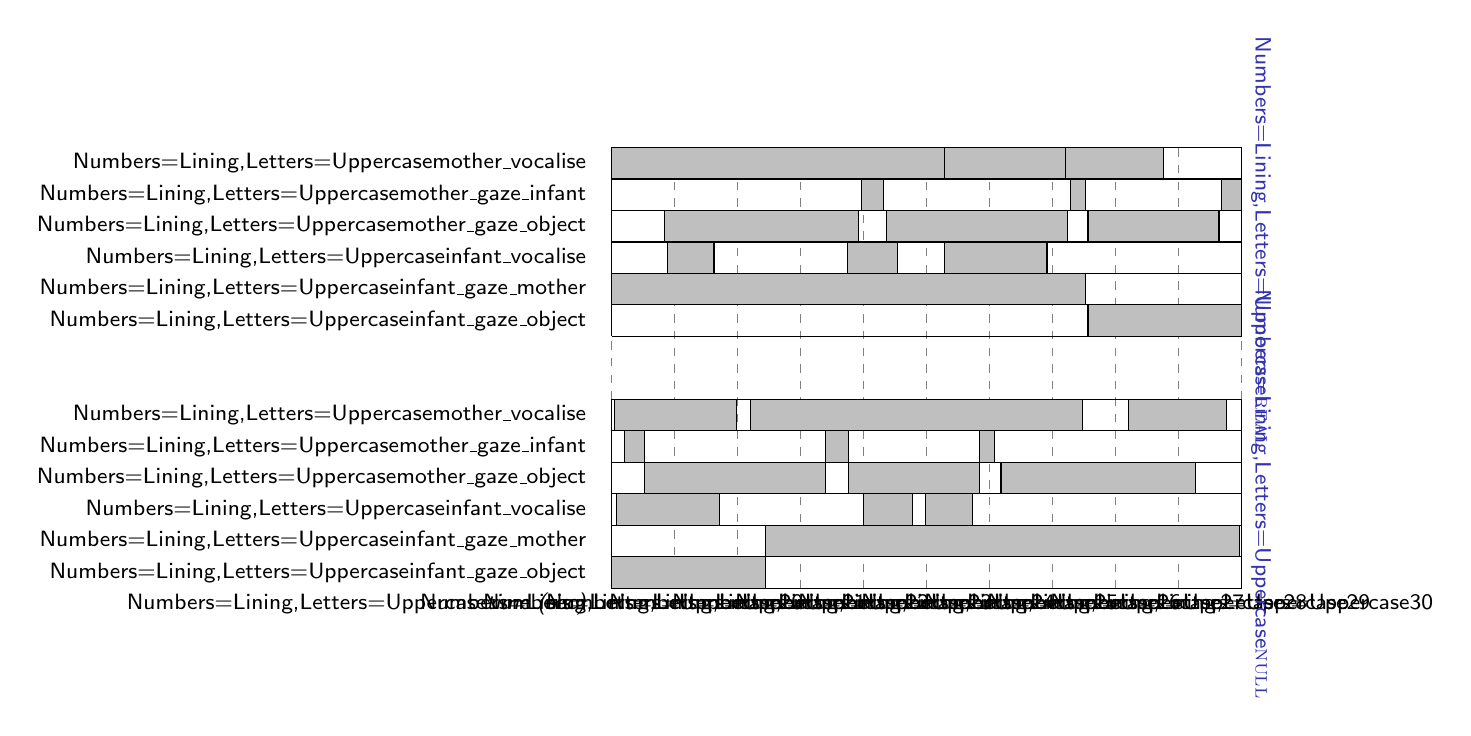
\begin{tikzpicture}[
	scale=0.8,  % a little smaller on beamer
	node distance=0 and 0,  % y, x for fuck knows what reason
	every node/.append style={font=\footnotesize\sffamily\addfontfeature{Numbers=Lining,Letters=Uppercase}}]
%	\draw [help lines] (0,0) grid (13,7);
	
	%% time line
	% annotations
	\node [anchor=east] at (2.75, -0.25) {\textit{time (sec)}};
	\foreach \i in {20, 21,..., 29, 30}
		\node at ({\i-17},-0.25) {\i};
	% small vertical help lines
	\draw [help lines, dashed] (3,3) -- (3,4);
	\draw [help lines, dashed] (13,3) -- (13,4);
	% long vertical help lines
	\foreach \i in {4, 5,..., 11, 12}
		\draw [help lines, dashed] (\i,0) -- (\i,7);
	
	%% grids
	% vertical lines
	\foreach \i in {3, 13}{
		\draw (\i,4) -- (\i,7);  % top
		\draw (\i,0) -- (\i,3);  % bottom
	}
	% horizontal lines
	\foreach \i in {0, 0.5,..., 2.5, 3, 4, 4.5,..., 6.5, 7}  % top and bottom
		\draw (3,\i) -- (13,\i);
	% annotations
	\node[color=beamerblue, rotate=-90, anchor=south] at (13,5.5) {\textsc{real}};
	\node[color=beamerblue, rotate=-90, anchor=south] at (13,1.5) {\textsc{null}};
		
	%% labels
	\foreach \i in {0.25, 4.25}{  % top and bottom
		\node[anchor=east] at (2.75,{\i+2.5}) {\code{mother\_vocalise}};
		\node[anchor=east] at (2.75,{\i+2}) {\code{mother\_gaze\_infant}};
		\node[anchor=east] at (2.75,{\i+1.5}) {\code{mother\_gaze\_object}};
		\node[anchor=east] at (2.75,{\i+1}) {\code{infant\_vocalise}};
		\node[anchor=east] at (2.75,{\i+0.5}) {\code{infant\_gaze\_mother}};
		\node[anchor=east] at (2.75,\i) {\code{infant\_gaze\_object}};
	}
	
	%% annotations
	% top
	\draw [fill=lightgray] (3,6.5) rectangle (8.279,7);
	\draw [fill=lightgray] (8.279,6.5) rectangle (10.206,7);
	\draw [fill=lightgray] (10.206,6.5) rectangle (11.76,7);

	\draw [fill=lightgray] (6.96,6) rectangle (7.32,6.5);
	\draw [fill=lightgray] (10.28,6) rectangle (10.52,6.5);
	\draw [fill=lightgray] (12.68,6) rectangle (13,6.5);
	
	\draw [fill=lightgray] (3.84,5.5) rectangle (6.92,6);
	\draw [fill=lightgray] (7.36,5.5) rectangle (10.24,6);
	\draw [fill=lightgray] (10.56,5.5) rectangle (12.64,6);
	
	\draw [fill=lightgray] (3.887,5) rectangle (4.624,5.5);
	\draw [fill=lightgray] (6.74,5) rectangle (7.53,5.5);
	\draw [fill=lightgray] (8.279,5) rectangle (9.909,5.5);
	
	\draw [fill=lightgray] (3,4.5) rectangle (10.52,5);

	\draw [fill=lightgray] (10.56,4) rectangle (13,4.5);
	% bottom
	\draw [fill=lightgray] (5.2,2.5) rectangle		({5.2+5.279},3);
	\draw [fill=lightgray] (3.05,2.5) rectangle		({3.05+1.927},3);
	\draw [fill=lightgray] (11.206,2.5) rectangle	({11.206+1.554},3);

	\draw [fill=lightgray] (6.4,2) rectangle		({6.4+0.36},2.5);
	\draw [fill=lightgray] (8.84,2) rectangle		({8.84+0.24},2.5);
	\draw [fill=lightgray] (3.2,2) rectangle		({3.2+0.32},2.5);
	
	\draw [fill=lightgray] (9.18,1.5) rectangle		({9.18+3.08},2);
	\draw [fill=lightgray] (3.52,1.5) rectangle		({3.52+2.88},2);
	\draw [fill=lightgray] (6.76,1.5) rectangle		({6.76+2.08},2);
	
	\draw [fill=lightgray] (7.987,1) rectangle		({7.987+0.737},1.5);
	\draw [fill=lightgray] (6.99,1) rectangle		({6.99+0.79},1.5);
	\draw [fill=lightgray] (3.079,1) rectangle		({3.079+1.63},1.5);
	
	\draw [fill=lightgray] (5.44,0.5) rectangle		({5.44+7.52},1);

	\draw [fill=lightgray] (3,0) rectangle			({3+2.44},0.5);
\end{tikzpicture}